% Prof. Dr. Ausberto S. Castro Vera
% UENF - CCT - LCMAT - Curso de Ci\^{e}ncia da Computa\c{c}\~{a}o
% Campos, RJ,  2022
% Disciplina: Paradigmas de Linguagens de Programa\c{c}\~{a}o
% Aluno: Rômulo Souza Fernandes


\chapter{Ferramentas existentes e utilizadas}

Neste capítulo será apresentadas algumas ferramentas para auxiliar no desenvolvimento em Python, algumas dessas ferramentas foram utilizadas até mesmo para realizar esse trabalho. A seguir algumas ferramentas separadas por categoria.
\begin{itemize}
  \item Nome da ferramenta (compilador-interpretador)
  \item Endere\c{c}o na Internet
  \item Vers\~{a}o atual e utilizada
  \item Descri\c{c}\~{a}o simples (m\'{a}x 2 par\'{a}grafos)
  \item Telas capturadas da ferramenta
  \item Outras informa\c{c}\~{o}es
\end{itemize}

    \section{Notepad++}
	O Notepad++ é um editor de texto de código aberto funcional e gratuito, reconhecendo diversas linguagens de programação, uma delas é o Python. Essa ferramenta também suporta vários idiomas. Sua última versão lançada é a Notepad++ v8.4.7, que está disponível para download gratuitamente no seu site oficial, o link a seguir fará o redirecionamento para a aba de downloads do \href{https://notepad-plus-plus.org/downloads/}{Notepad++}. 
	
	\begin{figure}[H]
		\begin{center}
			\caption{Ambiente de trabalho do Notepad++} \label{ling1}
			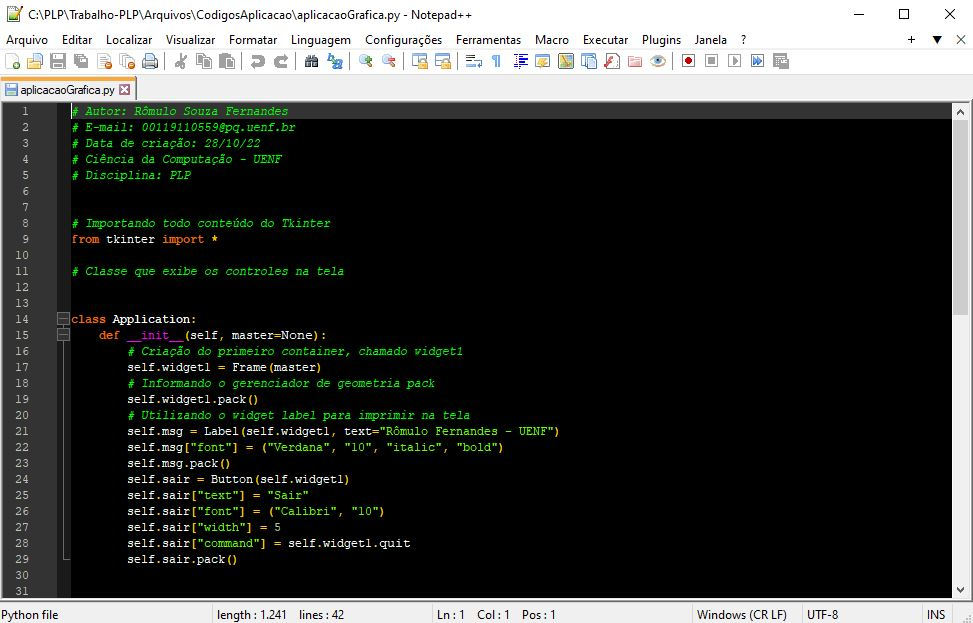
\includegraphics[width=6cm]{notepad.JPG} \\
			{\tiny \sf Fonte:{ Autor}}
		\end{center}
	\end{figure}
	
	Tem a utilização regida pela GNU General Public License. O Notepad++ é escrito em C++ e baseado no Scintilla. Possui alguns recursos muito úteis que são particulares, como a criação de atalhos para chamar programas, agrupa seções de código, permitindo a ocultação de blocos de código, deixando a janela mais legível.
	
     \section{Pycharm}
    
    \section{Visual Studio Code}
    
    
    \section{Compilador XYZ}


    \section{Interpretador Shell}
	%https://docs.python.org/pt-br/3/tutorial/interpreter.html
	%https://education.ti.com/html/webhelp/EG_TINspire/PT/Subsystems/EG_Python/Content/m_workspaces/ws_shell.HTML

   
    \section{Debug}
     